\documentclass[a4paper,11pt]{report}
\usepackage[italian]{babel}
\usepackage[utf8]{inputenc}
\usepackage[total={170mm,267mm},top=15mm,bottom=15mm,left=21mm,right=21mm]{geometry}
\usepackage{graphicx}
\usepackage[T1]{fontenc}
\usepackage{hyperref}
\usepackage{float}
\usepackage{fancyhdr}
\usepackage{amsmath}
\usepackage[dvipsnames]{xcolor}
\begin{document}

    \begin{titlepage}

        \clearpage\thispagestyle{empty}
        \centering
        \begin{figure}[h!]
            \begin{center}
                
\includegraphics[width=4cm]{img/logo1}\\
            \end{center}
        \end{figure}
        {\normalsize Informatica - Area scientifica \\  Dipartimento di Scienze matematiche, informatiche e multimediali\\  Università di Udine \par}
        \vspace{3cm}
        {\Huge \textbf{Seconda parte del progetto di ASD}\\
        \vspace{4cm}
            \begin{center}
                \Large
                Enrico Martin martin.enrico@spes.uniud.it 145175 \\
                Luca Bazzetto bazzetto.luca@spes.uniud.it 144760 \\
                Andrea Bordignon bordignon.andrea001@spes.uniud.it 142295
            \end{center}

            \vspace{9cm}
            {\normalsize Anno accademico 2020/2021}
            \pagebreak
        }
    \end{titlepage}

    \tableofcontents{}
    \pagebreak


    \chapter{Consegna}
    La seconda parte del progetto richiede l'implementazione e l'analisi dei tempi di l'esecuzione di operazioni di inserimento e di ricerca in alberi binari di ricerca. Nello specifico, si richiede di implementare le operazioni di ricerca e inserimento per tre tipi diversi di alberi binari di ricerca: alberi binari di ricerca semplici, di tipo AVL e di tipo Red-Black.
    \\Si assuma che ogni nodo di un albero binario di ricerca contenga una chiave numerica (di tipo intero) e un valore alfanumerico (di tipo stringa). Non è richiesta l'implementazione dell'operazione di rimozione di un nodo (i test automatici di auto-valutazione sono preparati in modo da non eseguire mai l'istruzione di rimozione).
    \vspace{2mm}
    \\Si richiede una stima dei tempi medi e ammortizzati per l'esecuzione di $n$ operazioni di inserimento e ricerca nei tre tipi di alberi binari di ricerca sopra descritti.
    \\Per tale stima si potrà procedere nel modo seguente:
    \\Al variare del parametro $n$, ad esempio, fra 1000 e 1000000, si eseguono $n$ volte le seguenti operazioni su un albero di ricerca inizialmente vuoto: si genera in modo pseudo-casuale un valore intero $k$, si ricerca un nodo con chiave $k$ nell'albero e, qualora il nodo non esistesse, si inserisce un nuovo nodo con chiave $k$ nell'albero. Si noti che al termine di tale procedura saranno state eseguite esattamente $n$ operazioni di ricerca e $m$ operazioni di inserimento, per un opportuno $m \le n$ (l'albero binario di ricerca conterrà quindi al più $n$ nodi). Nell'ipotesi che i numeri generati in modo pseudo-casuale varino in un dominio sufficientemente grande, il valore di $m$ sarà probabilmente simile a quello di $n$ e potrà quindi essere sostituito con $n$.
    \vspace{2mm}
    \\Si richiede di stimare il tempo ammortizzato al variare di $n$ con un errore relativo limitato superiormente da 0.01.


    \chapter{Approccio al progetto}
    ll primo approccio al progetto è stato quello di eseguire un'attenta lettura della consegna al fine di evidenziare in primis le varie richieste e contemporaneamente di effettuare una valutazione preliminare sugli obiettivi che sarebbero potuti risultare più difficili da implementare.\vspace{2mm}
    \\Successivamente è stato realizzato un diagramma, qui di seguito riportato, che sintetizza la metodologia globale con cui approcciarsi alla realizzazione del progetto.
    \\Il progetto infine è stato verosimilmente così svolto.
    \\Abbiamo, infatti, prima di tutto implementato i BST richiesti, successivamente testato la loro correttezza e una volta completati abbiamo poi calcolato la stima dei tempi medi e infine realizzato i grafici comparativi con le dovute scale.
    \begin{figure}[h!]
        \begin{center}
            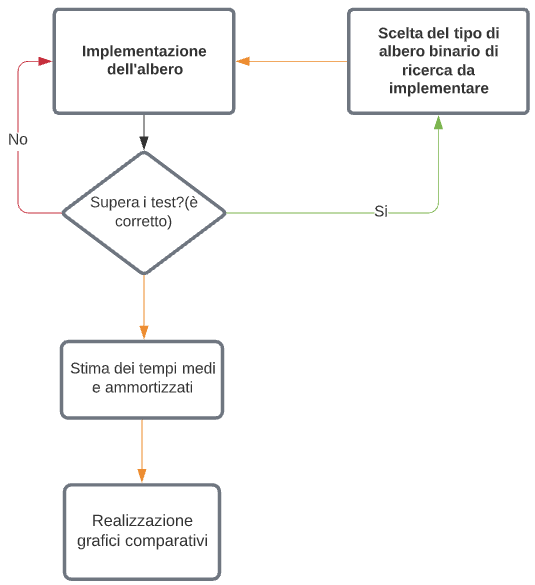
\includegraphics[width=120mm]{img/APP1}\\
        \end{center}
    \end{figure}


    \chapter{Analisi dei Tempi}
    In questa sezione della relazione si riporteranno i grafici delle misurazioni dei tempi.
    \\I tempi sono stati misurati per ogni albero binario in 100 differenti esecuzioni. %in funzione dell'input??
    \\I grafici mettono sempre in relazione i tre alberi binari di ricerca distinti dai seguenti colori:
    \begin{itemize}
        \item {\color{Red}{Rosso}}: AVL
        \item {\color{Blue}{Blu}}: BST
        \item {\color{Green}{Verde}}: RBT
    \end{itemize}


    \section{Grafico 1}
    Il primo grafico mostra l'andamento logaritmico crescente in funzione della dimensione dell'input dei tre algoritmi in funzione di n.
    \\Nell’asse delle ascissa troviamo $n$ -la dimensione dell'input- mentre nell’ordinata troviamo il tempo espresso in secondi.
    \\Si notano poi diversi valori dall'andamento altalenante -non costante- sopratutto nella fase iniziale, traducibili in termini di costi di overhead.\\

    \begin{figure}[h!]
        \begin{center}
            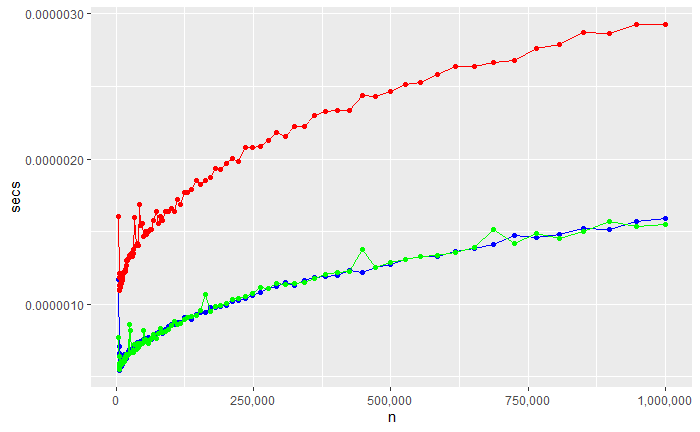
\includegraphics[width=16cm]{img/giusto1}\\
        \end{center}
    \end{figure}
    \pagebreak


    \section{Grafico 2}
    In questo secondo grafico è stata applicata una scala logaritmica per ogni asse. Questo fa risultare i campioni distribuiti in maniera uniforme, tuttavia rimane coerente con il grafico precedente e ci permette di capire quale dei tre algoritmi sia il più efficiente e, ovviamente, quale il meno.
    \vspace{0,5cm}
    \\La lettura del grafico infatti ci permette di ordinare gli algoritmi in termini di efficienza (dal più vantaggioso al meno) e stilarne la seguente "classifica":
    \begin{itemize}
        \item 1. {\color{Blue}{BST}}
        \item 2. {\color{Green}{RBT}}
        \item 3. {\color{Red}{AVL}}
    \end{itemize}
    Si osserva anche che gli algoritmi  {\color{Blue}{BST}} e {\color{Green}{RBT}} differiscono di poco e non è immediato riconoscere quale dei due sia più efficiente rispetto all'altro.
    \\Immediato è invece il distacco con {\color{Red}{AVL}}.
    \begin{figure}[h!]
        \begin{center}
            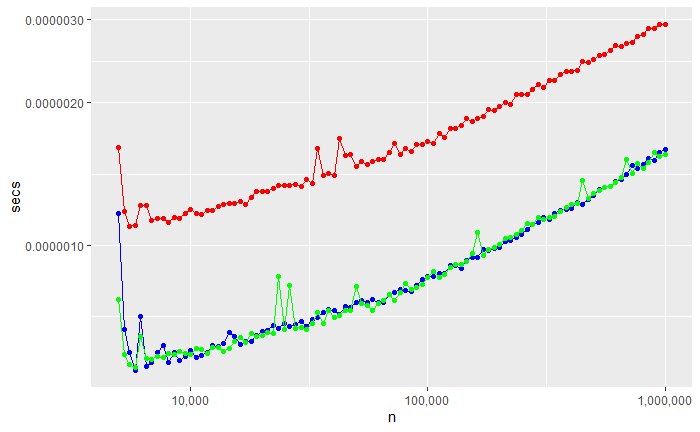
\includegraphics[width=17cm]{img/giusto2}\\
        \end{center}
    \end{figure}


    \chapter{Conclusioni}
    I tre algoritmi, come già riportato, presentano un andamento logaritmico. Essendo nota la teoria dei seguenti alberi binari di ricerca ritroviamo una certa coerenza -in termini di implementazione e di misurazione dei tempi- nel momento in cui il loro andamento rispecchia la loro complessità asintotica nel caso medio, ovvero: $O(log(n))$.
% dire che in linea teorica verde dovbrebbe essere meglio(?)
    \\Riportiamo inoltre i calcoli della media e della deviazione standard per ogni algoritmo:
    \begin{itemize}
        \item {\color{Blue}{BST}}
        \begin{itemize}
            \item \textbf{media:} 0.0000894534
            \item \textbf{deviazione standard:} 0.0000000001
        \end{itemize}
        \item {\color{Red}{AVL}}
        \begin{itemize}
            \item \textbf{media:} 0.0001737295
            \item \textbf{deviazione standard:} 0.0000000003
        \end{itemize}
        \item {\color{Green}{RBT}}
        \begin{itemize}
            \item \textbf{media:} 0.0000894632
            \item \textbf{deviazione standard:} 0.0000000001
        \end{itemize}
    \end{itemize}
    In conclusione decretiamo l'algoritmo BST come più vantaggioso , d'altra parte è l'algoritmo AVL a rivelarsi come meno vantaggioso.
    \\Inoltre i risultati della deviazione standard per i due algoritmi più efficienti ci danno un riscontro di un uniformità di valori migliore rispetto al restante algoritmo.
\end{document}\\